\chapter{Biomass functions and nutrient contents of European beech, oak, sycamore maple and ash and their meaning for the biomass supply chain}
\label{chap:bm}
{\large Kai Husmann$^1$ - Sabine Rumpf$^2$ - J�rgen Nagel$^2$}\\

\vspace{3cm}
\noindent
$^1$Department of Forest Economics and Forest Management,\\ University of G�ttingen, B�sgenweg 3, 37077 G�ttingen, Germany \\

%\vspace{0.5cm}
\noindent
$^2$Northwest German Forest Research Institute,\\ Gr�tzelstra�e 2, 37079 G�ttingen, Germany\\

\vspace{\fill}
\noindent
Published in:\\
Journal of Cleaner Production.\\(DOI: X)

\newpage
\begin{itemize}
	\item Sabine Rumpf performed the nutrient efficiency analysis and coordinated the field work.
	\item J�rgen Nagel supported writing of the manuscript and the review process.
\end{itemize}

\cleardoublepage
%%%%%%%%%%%%%%
%% Abstract %%
%%%%%%%%%%%%%%
\section*{Abstract}
\label{chap:bm:Abstract}
Woody biomass from forests has great potential to provide a continuous and largely carbon-neutral raw material supply for the bio-based industry. As the demand for forestry products is already very high and steadily increasing, the question arises how to match the limited available wood resources to the growing demand for raw materials. Thus, there is an initial need to properly estimate the available biomass from forests. The success of a bio-based industry depends on an accurate forecast of the raw material flow coming from the forests for the entire biomass supply chain up to the industrial processing stage. Using easily measured input data, e. g. the tree diameter at breast height, biomass functions allow for a reliable prediction of tree species- and tree fraction-specific single-tree biomasses. In combination with nutrient content data, the site specific ecologically sustainable level of forestry use can be assessed and the site-specific wood utilization potential can be fully exploited.
Biomass functions for the main tree species can be found in the literature. For other tree species, like sycamore or ash, however, there are only very specific studies available. As the wood potential of especially those species is recently often unused, goal of this study is to develop biomass functions and nutrient contents for European beech, oak, ash and sycamore for the fractions stem wood, bark, branches, and twigs.\\

For this purpose 139 trees were destructively sampled. Their single tree biomasses and nutrient contents were examined. This data was then used in a regression analysis to build generalized tree species- and tree fraction-specific biomass functions and nutrient contents for northern and central Germany.
We showed that the sycamore and ash biomass functions differed significantly from those of European beech and oak. Using oak biomass functions for the biomass estimation of sycamore and ash, as it is practiced today, leads to a massive overestimation of the standing biomass in a test site up to 11 \% (21 tons / ha respectively).\\

The share of species-rich broadleaf forest stands, and thereby the importance of tree specific biomass functions, is increasing. The introduced models can help to exploit the huge biomass potential of those deciduous stands.\\

\subsection*{Keywords}
Biomass function - Nutrient content - Long-living tree species - Biomass supply chain - Site sustainability

\subsection*{Highlights}
\begin{itemize}
\item Effectivity of biomass supply chains depend on reliable biomass estimation.
\item The wood potential of long-living tree species is recently often unused.
\item Biomass models for sycamore maple and ash can help gathering this potential.
\end{itemize}
%%%%%%%%%%%%%%%%%%
%% Introduction %%
%%%%%%%%%%%%%%%%%%
\section{Introduction}
\label{sec:bm:Introduction}

Biomass from forests has real potential to provide a continuous and largely carbon-neutral supply of material to the bio-based industry sector and can therefore make a significant contribution to a clean bio-based industry. Especially small dimensioned wood has huge potential for use in bio-refineries. \citet{ekman_2013} showed in Sweden that previously unused scrap wood can be used for the extraction of high quality chemical substances, such as bio-oils or antioxidants for use in the food or cosmetics industries. Supply of biomass from forestry can drive the economic growth of the entire bio-based chemical industry and make it competitive in the long-term, especially if wood fractions that have up to now been used as fuel wood are included. Innovative industries, such as the nanofiber or biochemistry industries, are increasing the demands on the forestry product-pool. The forest-based bio-economy is already an integral part of the global forestry sector \citep{hurmekoski_2013}. The European bio-based industry is currently a growing sector, with Germany playing a leading role \citep{hennig_2016}.

The global forestry industry is currently undergoing a process of change. The use of wood as raw materials in Germany has increased considerably in the last decades \citet{mantau_2012}. Changes in government energy policy and the development of new technology led to development of new markets, in particular for small dimensioned wood \citep{geldermann_2016, mccormick_2013}. The demand for forestry products is steadily rising, increasing the competition for raw timber. The question then is how to match the available wood resource to the demand for raw materials.

Just as it is for classical forestry \citep{mohring_1997}, knowledge of the available potential biomass is the main prerequisite for a functioning bio-based industry \citep{hennig_2016}. Using wood means that the nutrients bound in the wood are removed from the forest ecosystem. The biomass potential of a forest can only be utilized to an extent that, in the long-term, won�t deplete the supply of plant available nutrients in the forest ecosystem. In order to be able to exploit the woody biomass potential for the bio-based industry, the limit of the utilisation extend from the forests stands must be known \citep{block_2013, pretzsch_2014}. Therefore, reliable estimates of the quantity of biomass to be harvested, as well as reliable estimates of the amount of nutrients contained in these biomasses are required.

Using easily measured input data, such as diameter at breast height (dbh) or tree height, biomass functions enable the prediction of single-tree biomasses. Tree species and tree-fraction specific estimations of the forest biomass supply can be made. Using these biomass functions coupled with nutrient content data, the nutrient export can be estimated. In this way an ecologically sustainable level of forestry use can be calculated and the site specific wood utilization potential can be fully exploited.

The success of the bio-based industry depends to a great extent on the ability to accurately forecast the flow of raw materials in the integrated biomass supply chain \citep{geldermann_2016, how_2016}. Using biomass functions the relevant information for strategic operational decision-making can be generated for the entire biomass supply chain - from the forest stand to the industrial processing stage. Detailed biomass calculations can improve planning certainty along the entire value chain because the masses to be transported and those due at the factory gate can be forecasted very accurately. Biomass functions can therefore make an important contribution to increasing the planning capability, and thereby to cost reductions, in operative planning for forestry enterprises, wood logistics and wood industry firms.

Wood industry cluster studies on the availability of raw materials and on the market situation of the wood industry are the bases for the strategic orientation of the bio-economy industries \citep{mccormick_2013}. By using supply analyses and material flow simulations together with biomass functions decision support models can be parameterised which enable, for example, the computing of a continuous biomass supply chain \citep[e. g.][]{ruther_2007, wordehoff_2011, mantau_2012}.

Responsible biomass usage from forests has, next to its economic relevance, also very important social impacts. In 2006, under the terms of the Kyoto protocol, reporting of the carbon sequestration performance of forests became mandatory in Germany. The use of biomass functions is an integral part of this reporting process \citep{vallet_2006, tabacchi_2011, wordehoff_2011}.

In the literature there are numerous biomass functions \citep[e. g.][]{grote_2003, cienciala_2005, pretzsch_2014} and nutrient content figures \citep[e. g.][]{augusto_2000, jacobsen_2003, weis_2012, pretzsch_2014} available for the tree species European beech (Fagus sylvatica [L.]), common oak (Quercus robur [L.]) and sessile oak (Quercus petraea [L.]). For sycamore maple (Acer pseudoplatanus [L.]) and ash (Fraxinus excelsior [L.]) however, there are only few functions available. All literature functions found either do not cover the entire relevant diameter spectrum \citep[e. g.][]{albert_2014, alberti_2005} or do not allow fraction specific biomass estimation \citep{bunce_1968}.

The wood increment of long-term deciduous trees, which is the species group sycamore and ash belong to, was only used by 38 \% between 2002 and 2012 \citep{ti_2014}. This is certainly partially reasoned by the fact that reliable planning methods for long-term deciduous species are not available. The question then arises if the predictions of the woody biomass in these stands could be improved by using specific biomass functions and nutrient contents for sycamore and ash. Specific biomass functions for these species could help making the recently unused potential available for the bio-based industry.

The goal of this study is to develop biomass functions for European beech, oak, sycamore and ash by means of regression analysis, using data gathered in northern and central Germany. Functions are developed for the tree fractions stem wood (diameter > 7cm without bark), bark of stem wood, branches (1 - 7cm with bark), and twigs (< 1cm with bark). The differences in these biomass functions are examined at single-tree and stand level by means of a sensitivity analysis in an exemplary test stand. The nutrient content in the different tree fractions of the tree species studied are determined and used as the basis for quantifying the nutrient removal by harvesting. The amount of nutrients that are removed from the forest ecosystem is then determined by multiplying the nutrient content with the biomass.

%%%%%%%%%%%%%%%%%%%%%%%%%%%
%% Materials and Methods %%
%%%%%%%%%%%%%%%%%%%%%%%%%%%
\section{Materials and Methods}
\label{sec:bm:methods}
With the goal of quantifying biomass and nutrient content 139 vital trees were studied (Table \ref{tab:bm:tab1}). The sample plots for beech and oak represented as many different growing areas and site conditions as possible. The high nutrient requirements of sycamore and ash meant that the sample plots for these species were exclusively on nutrient-rich, calcareous substrates. Per plot 2 - 4 trees were chosen (Figure \ref{fig:bm:fig1}). Both within each sample site, and across the plots as a whole, the aim was to collect trees from a wide and evenly distributed diameter range.

\begin{figure}
	\center
	\includegraphics[width=0.75\textwidth]{Grafiken/bm/Fig_1_Locations.eps}
	\caption{Locations of the 54 sampled plots. Source of the background map: \citet{facg_2014}.}
	\label{fig:bm:fig1}
\end{figure}

% Please add the following required packages to your document preamble:
% \usepackage{multirow}
\begin{table}[]
	\centering
	\caption{Descriptive statistics of the sampled trees.}
	\label{tab:bm:tab1}
	\begin{tabular}{cccccc}
		\cline{1-6}
		\multicolumn{1}{l}{}    &                          & oak   & \begin{tabular}[c]{@{}c@{}}European\\ beech\end{tabular} & ash   & sycamore \\ \cline{1-6}
		\multicolumn{1}{l}{}    &     number of trees             & 40   & 37 & 37   & 25 \\ \cline{1-6}
		
		\multirow{4}{*}{dbh {[}cm{]}}    & minimum     & 8.00  & 8.00                                                    & 9.10  & 12.00    \\
		&  mean        & 35.40 & 32.50                                                   & 31.90 & 28.20    \\
		&  std. dev.   & 23.70 & 17.14                                                   & 17.30 & 10.40    \\
		&  maximum     & 95.40 & 66.40                                                   & 75.60 & 56.10    \\ \cline{1-6} 
		\multirow{4}{*}{height {[}m{]}} &  minimum   & 9.60  & 15.30                                                   & 14.40 & 15.20    \\
		&  mean      & 22.10 & 24.90                                                   & 25.60 & 22.60    \\
		& std. dev. & 6.90  & 6.65                                                    & 6.70  & 4.25     \\
		&  maximum   & 32.00 & 35.25                                                   & 38.50 & 31.80    \\ \cline{1-6} 
		\multirow{4}{*}{age {[}a{]}}    &  minimum      & 25    & 21                                                      & 34    & 33       \\
		&  mean         & 86    & 84                                                      & 74    & 51       \\
		&  std. dev.    & 54    & 44                                                      & 37    & 23       \\
		& maximum      & 190   & 180                                                     & 153   & 118      \\ \cline{1-6} 
	\end{tabular}
\end{table}
%%-------------------------------------%%
%% Data sampling and sample processing %%
%%-------------------------------------%%
\subsection{Data sampling and sample processing}
\label{subsec:bm:methods:sampling}

Dbh, height at crown base and tree height were measured for each tree. The fraction volumes of the trees were determined using randomized branch sampling (RBS). RBS is an efficient and bias free sampling method for estimating tree fractions \citep{saborowski_1999, Gregoire_2008}. Since this method was firstly described \citet{jessen_1955} it has been used in other studies, including those from \citet{valentine_1984}, \citet{gaffrey_1999} and \citet{affleck_2015}. This multi-stage sampling method assumes proportionality between the target quantity and an easily measurable proxy. Because an allometric relationship exists between branch volume and branch base diameter \citep{west_1999}, the RBS method makes it possible to estimate the wood volume by measuring only a subset of branch lengths and branch diameters in the tree crowns. The stem form was assessed by section-wise diameter measurements at certain tree heights up to the crown base. In order to determine the specific bulk density and nutrient contents, up to 12 samples, covering all diameters of the tree, were collected per tree using the Importance Sampling \citep{Gregoire_2008}.

Half of the samples were measured and weighted in fresh state and, after several days drying at 103 �C, in absolute dry condition in order to determine the bulk density [kg biomass (dry) / m$^3$ wood volume (fresh)] \citep{rademacher_2011}. For all stem wood samples (diameter > 7cm) the bark was separated from the wood before drying. From this samples tree species and tree fraction specific bulk density coefficients were calculated. The fraction volumes, which were previously estimated using the RBS method, could then be converted into biomasses using these bulk density coefficients. The other half of the samples underwent a chemical analysis in order to determine their nutrient concentrations. In our sample preparation and analysis we followed the widely used method by \citet{konig_2012a, konig_2012b}. In order to ensure comparability between all studied tree species, only European beech and oak samples from sample plots on nutrient-rich substrates were considered for the chemical analysis.

%%-------------------%%
%% Biomass functions %%
%%-------------------%%
\subsection{Biomass functions}
\label{subsec:bm:methods:bm_functions}

In order to parameterize tree species and tree fraction dependent biomass functions the single-tree biomass information was analyzed by regression analysis. The biomass functions were estimated using nonlinear Generalized Least Squares Estimation. The exponential function used in \citet{hochbichler_2006} (Equation \ref{eq:bm:eq1}) was chosen as the model type \citep{rumpf_2011}. The validity of each model was tested via visual analysis of the weighted model residuals including a comparison with theoretical residuals (quantile-quantile-analysis). Furthermore the bias of each model was calculated as the mean of the model residuals.

\begin{equation}
\label{eq:bm:eq1}
\hat{Y}_i=\exp{\left(\alpha+\beta \, ln(dbh_i)+\gamma \, ln(h_i)\right)}\,\varepsilon_i
\end{equation}

One general assumption in regression analysis is the independence of the model errors $\varepsilon_i$. Because this assumption is probably not met for the tree fractions within a tree species, a model distortion due to correlation between the covariates (collinearity) is possible. Not taking this collinearity into account can influence the results of a regression and thereby limit the model validity \citep{graham_2003}. In order to estimate the magnitude of the error resulting from collinearity, in addition to the single model variances $var(\hat{y}_i)$, combined model variances per tree species $\hat{\bar{y}}$ were calculated \citep{parresol_2001}. This combined model variance per tree species consists of the single model variances $var(\hat{y}_i)$ and the model co-variances $cov(\hat{y}_i, \hat{y}_j)$ between the fraction functions for a respective tree species (Equation \ref{eq:bm:eq2}). The correlation between two fractions  was estimated using a linear correlation coefficient of the measured biomasses.

\begin{equation}
\label{eq:bm:eq2}
var(\hat{\bar{y}}_i)={wait} {for} {proof}
\end{equation}

The multiplicative error term $\varepsilon_i$ of the nonlinear biomass function (Equation \ref{eq:bm:eq2}) implies an increasing variance with increasing covariate dimension. We quantified the resulting heteroscedasticity by parameterizing a power function with the model residuals over the fitted values. This function was then used to weight the residuals of the actual fit. Thus, neither the variances of the distinct biomass functions $var(\hat{y}_i)$ nor the combined model variance $var(\hat{\bar{y}}_i)$ showed heteroscedasticity.

In order to make the single model variances $var(\hat{y}_i)$ comparable to each other, to the variances of other biomass functions in the literature and to the combined model variances per tree species $var(\hat{\bar{y}}_i)$, dimensionless coefficients of variation for each model $i$ were calculated (Equation \ref{eq:bm:eq3}), where $j$ is the index for the observed tree. These coefficients of variation were also calculated for the combined model error $v(\hat{\bar{y}}_i)$. $v(\hat{y}_i)$ and $v(\hat{\bar{y}}_i)$ thus represent the normalized deviation of the models. They are calculated as the quotient of the deviation and the estimated response. This normalization is advantageous since it scales every residuum by its expected dimension thereby making it easily interpretable and comparable. The absolute deviation would, due to the heteroscedasticity, increase with increasing dimension of the response $y_{ij}$.

\begin{equation}
\label{eq:bm:eq3}
var(\hat{\bar{y}}_i)={wait} {for} {proof}
\end{equation}

where $i$ denotes the fraction and $j$ the observed tree. $N_i$ is the number of observations in fraction $i$. The entire regression analysis was performed using with the R package \textit{nlme} \citep{venables_2002}. Additionally, we calculated the likelihood-ratio based pseudo-r-squared for each model using \textit{MuMIn} \citep{barton_2016}.

To enable a comparison between the biomass functions for the different tree species 95 \% confidence intervals were computed for European beech and oak using bootstrapping \citep{diciccio_1996}. To do this every regression model for these two species was repeated 1,000 times using sub-samples of the original data which were selected randomly by drawing with replacement. In order to prevent the sample size influencing the width of the confidence intervals, the number of samples in every repetition matched the actual number of samples. All analyses were performed using the R software \citet{r_core_team_2016}.

%%----------------------%%
%% Sensitivity analysis %%
%%----------------------%%
\subsection{Sensitivity analysis}
\label{subsec:bm:methods:sensitivity}
To analyze the behavior of our models, the biomass functions were applied on a real forest site. This site was chosen for testing purposes only. The trees of the site were not included in the regression analyses. The research site is located ca. 15 km east of the city of G�ttingen. It is a mixed stand with European beech, sycamore and ash, which is typical for this region. The site is on a sun exposed slope with a stony substrate consisting of the products of limestone weathering overlain by a thin layer of loess (Table \ref{tab:bm:tab2}). It has a good nutrient and a good water supply.

\begin{table}[]
	\centering
	\caption{Tree layer specific parameters of the test site. Growth region: Middle German Trias High and Hill Land. Growth district: G�ttingen Forest. Altitude: 340 m. hm: Height of stem of mean basal area. dm: Diameter of stem of mean basal area.}
	\label{tab:bm:tab2}
	\begin{tabular}{ccccc}
		\hline
		tree species   & age & \begin{tabular}[c]{@{}c@{}}hm \\ {[}m{]}\end{tabular} & \begin{tabular}[c]{@{}c@{}}dm \\ {[}cm{]}\end{tabular} & \begin{tabular}[c]{@{}c@{}}stand volume \\ {[}m$^3$ ha$^{-1}${]}\end{tabular} \\ \hline
		European beech & 76  & 23.3                                                  & 27.6                                                   & 164.0                                                               \\
		European beech & 20  & 14.9                                                  & 11.2                                                   & 4.8                                                                 \\
		ash            & 71  & 28.7                                                  & 35.2                                                   & 73.3                                                                \\
		sycamore       & 76  & 24.3                                                  & 23.6                                                   & 18.7                                                                \\ \hline
	\end{tabular}
\end{table}

Based on this test site, 5 simulated test sites, differing in their species composition, were generated. For this, the proportions of the 3 tree species in the real stand were modified using the \textit{WaldPlaner} forest simulator \citep{hansen_2014}. With this software we randomly cloned original trees from the test site until the target mix ratio was achieved.
%%-------------------%%
%% Nutrient contents %%
%%-------------------%%
\subsection{Nutrient contents}
\label{subsec:bm:methods:nutrients}
To consider site sustainability is to ask the question - how to best manage the scarce nutrient resources available? To do this, the nutrient response efficiencies of the distinct species and fractions appear to be a reasonable \citep{henderson_2012}. The nutrient response efficiency \citep{vitousek_1982} tells us how much carbon [kg] can be bound by a plant per 1 kg of applied nutrients. According to \citet{vitousek_1982}, we define the response efficiency as the inverse of the element concentration of the biomass. It is the ratio of carbon to the other mineral nutrients. The tree and fraction specific nutrient response efficiency of each nutrient is thus calculated by dividing the carbon concentration by the respective nutrient concentration in the tree fractions. It determines how much nutrient must be assimilated to grow a certain amount of biomass. Trees with high nutrient response efficiency need less nutrients to grow the same amount of biomass in the respective fraction than a plant with lower nutrient response efficiency. The total tree nutrient response efficiency was calculated by dividing the total tree concentration of carbon, the sum of all 4 fractions, by the total concentration of the respective nutrient. From the samples that were chemically tested, the average nutrient response efficiencies per tree species and were calculated. This was achieved by calculating the mean nutrient response efficiencies per tree species from the single-tree values.

%%%%%%%%%%%%%
%% Results %%
%%%%%%%%%%%%%
\section{Results}
\label{sec:bm:results}

%%-------------------%%
%% Biomass functions %%
%%-------------------%%
\subsection{Biomass functions}
\label{subsec:bm:results:bm_functions}

The numbers of parameters in the biomass functions were determined by Akaike Information Criterion (AIC) \citet{akaike_1981}. By including tree height in the models for stem wood and bark the AIC scores were lowered markedly. This was observed for all species. In those cases, where tree height had a significant influence on the biomass, additional models were calculated with the dbh as the only independent variable. As a consequence of this, for each of the tree species there is an easily applicable dbh model available for each function. The coefficients of variation $v(\hat{\bar{y}}_i)$ and $v(\hat{y}_i)$ allowed a direct comparison of the single and the combined variances. In those cases in which the tree height coefficient was significant the model coefficients of variation were markedly reduced by its inclusion. The coefficients of variation fall into two groups (Table \ref{tab:bm:tab3}). The coefficients of variation for the functions of stem wood and bark of the stem wood are clearly smaller than those for branches and twigs. Even if the height is not included $v(\hat{y}_i)$ of the stem wood and bark models is substantially smaller than $v(\hat{y}_i)$ of the branches and twigs.

\begin{table}[]
	\centering
	\caption{Coefficients and standard deviation of the biomass functions (Equation \ref{eq:bm:eq1}) for the tree species European beech, oak, ash and sycamore including a combined model error (Equation \ref{eq:bm:eq2}) for each species. $v(\hat{y}_i)$: Coefficient of variation. $r^{2}_{LR}$: likelihood-ratio based pseudo-r-squared.}
	\label{tab:bm:tab3}
	\begin{tabular}{ccccccccc}
		\hline
		species  & N  & fraction          & $\alpha$             & $\beta$      & $\gamma$     & AIC   & $v(\hat{y}_i)$     & $r^{2}_{LR}$     \\ \hline
		oak      & 41 & \multicolumn{2}{c}{combined model error} &              &              &       & 0.040 &       \\ \hline
		&    & stem wood         & -5.6509              & 1.9222       & 1.6316       & 435.9 & 0.039 & 0.998 \\
		&    &                   & ($\pm$0.354)         & ($\pm$0.102) & ($\pm$0.211) &       &       &       \\
		&    & bark              & -6.3130              & 1.7037       & 1.5738       & 310.3 & 0.039 & 0.997 \\
		&    &                   & ($\pm$0.348)         & ($\pm$0.102) & ($\pm$0.209) &       &       &       \\ \cline{3-9} 
		&    & stem wood         & -2.8992              & 2.5924       &              & 468.2 & 0.050 & 0.997 \\
		&    &                   & ($\pm$0.205)         & ($\pm$0.057) &              &       &       &       \\
		&    & bark              & -3.6611              & 2.3505       &              & 340.7 & 0.049 & 0.995 \\
		&    &                   & ($\pm$0.201)         & ($\pm$0.056) &              &       &       &       \\
		&    & branch            & -1.3987              & 1.5827       &              & 377.1 & 0.131 & 0.975 \\
		&    &                   & ($\pm$0.332)         & ($\pm$0.114) &              &       &       &       \\
		&    & twig              & -3.1298              & 1.6758       &              & 307.9 & 0.201 & 0.891 \\
		&    &                   & ($\pm$0.657)         & ($\pm$0.201) &              &       &       &       \\ \hline
		beech    & 38 & \multicolumn{2}{c}{Combined model error} &              &              &       & 0.036 &       \\ \hline
		&    & stem wood         & -4.5238              & 2.1778       & 1.0373       & 414.5 & 0.037 & 0.996 \\
		&    &                   & ($\pm$0.393)         & ($\pm$0.088) & ($\pm$0.196) &       &       &       \\
		&    & bark              & -6.0328              & 1.9511       & 0.9515       & 221.1 & 0.035 & 0.995 \\
		&    &                   & ($\pm$0.362)         & ($\pm$0.080) & ($\pm$0.183) &       &       &       \\ \cline{3-9} 
		&    & stem wood         & -2.5687              & 2.5852       &              & 438.1 & 0.049 & 0.993 \\
		&    &                   & ($\pm$0.193)         & ($\pm$0.056) &              &       &       &       \\
		&    & bark              & -4.2350              & 2.3230       &              & 242.2 & 0.043 & 0.992 \\
		&    &                   & ($\pm$0.175)         & ($\pm$0.051) &              &       &       &       \\
		&    & branch            & -1.1673              & 1.5580       &              & 349.5 & 0.117 & 0.897 \\
		&    &                   & ($\pm$0.340)         & ($\pm$0.110) &              &       &       &       \\
		&    & twig              & -3.4372              & 1.6993       &              & 282.5 & 0.283 & 0.802 \\
		&    &                   & ($\pm$0.839)         & ($\pm$0.271) &              &       &       &       \\ \hline
		ash      & 37 & \multicolumn{2}{c}{Combined model error} &              &              &       & 0.026 &       \\ \hline
		&    & stem wood         & -4.3728              & 1.9730       & 1.1765       & 374.2 & 0.023 & 0.999 \\
		&    &                   & ($\pm$0.157)         & ($\pm$0.050) & ($\pm$0.092) &       &       &       \\
		&    & bark              & -6.8483              & 1.9737       & 1.2909       & 256.8 & 0.032 & 0.997 \\
		&    &                   & ($\pm$0.341)         & ($\pm$0.092) & ($\pm$0.180) &       &       &       \\ \cline{3-9} 
		&    & stem wood         & -2.4182              & 2.5144       &              & 426.9 & 0.039 & 0.996 \\
		&    &                   & ($\pm$0.189)         & ($\pm$0.053) &              &       &       &       \\
		&    & bark              & -4.3601              & 2.4730       &              & 289.4 & 0.045 & 0.994 \\
		&    &                   & ($\pm$0.237)         & ($\pm$0.064) &              &       &       &       \\
		&    & branch            & -2.1015              & 1.8858       &              & 330.7 & 0.074 & 0.969 \\
		&    &                   & ($\pm$0.286)         & ($\pm$0.087) &              &       &       &       \\
		&    & twig              & -3.3426              & 1.6436       &              & 242.0 & 0.174 & 0.857 \\
		&    &                   & ($\pm$0.657)         & ($\pm$0.204) &              &       &       &       \\ \hline
		\multicolumn{9}{c}{To be continued on following page.}
	\end{tabular}
\end{table}

\begin{table*}[]
	\centering
	\caption*{Table \ref{tab:bm:tab3} (continued)}
	\begin{tabular}{ccccccccc}
		\hline
		species  & N  & fraction          & $\alpha$             & $\beta$      & $\gamma$     & AIC   & $v(\hat{y}_i)$     & $r^{2}_{LR}$     \\\hline
		sycamore & 25 & \multicolumn{2}{c}{Combined model error} &              &              &       & 0.039 &       \\ \hline
		&    & stem wood         & -4.1220              & 2.0364       & 0.9797       & 225.1 & 0.029 & 0.997 \\
		&    &                   & ($\pm$0.274)         & ($\pm$0.082) & ($\pm$0.163) &       &       &       \\
		&    & bark              & -5.8308              & 1.8880       & 0.9918       & 118.2 & 0.030 & 0.996 \\
		&    &                   & ($\pm$0.274)         & ($\pm$0.083) & ($\pm$0.165) &       &       &       \\ \cline{3-9} 
		&    & stem wood         & -2.4235              & 2.4461       &              & 249.5 & 0.046 & 0.992 \\
		&    &                   & ($\pm$0.215)         & ($\pm$0.064) &              &       &       &       \\
		&    & bark              & -4.1984              & 2.3299       &              & 141.9 & 0.047 & 0.991 \\
		&    &                   & ($\pm$0.212)         & ($\pm$0.064) &              &       &       &       \\
		&    & branch            & -3.5005              & 2.1777       &              & 211.7 & 0.160 & 0.916 \\
		&    &                   & ($\pm$0.593)         & ($\pm$0.190) &              &       &       &       \\
		&    & twig              & -5.6275              & 2.3005       &              & 147.9 & 0.252 & 0.893 \\
		&    &                   & ($\pm$0.932)         & ($\pm$0.298) &              &       &       &       \\ \hline
		
\end{tabular}
\end{table*}

Altogether $v(\hat{y}_i)$ ranged from 0.02 to 0.28. With values between 0.03 and 0.04, the combined model coefficients of variation when collinearity is taken into account (Equation \ref{eq:bm:eq2}) were always small. The combined $v(\hat{\bar{y}}_i)$ were calculated from the respective best models (the models with height parameter for stem wood and bark). The combined model coefficients for the European beech, oak and ash models were very close to the coefficients for stem wood and stem wood bark. Although there were correlations between fractions, these were higher for models with low variance. Accordingly the combined model coefficients of variation for European beech, oak and ash were low. Only the sycamore model showed considerable difference between the combined model variation coefficients and the variation coefficients of stem wood and bark of the stem wood. This is explained by the relatively high correlation between the stem wood biomass with the branch and twig biomasses. Despite this, because the coefficients of variation for the sycamore stem wood and bark models are relatively low, the combined model coefficients of variation are approximately the same as those for European beech and oak. As the residuals of each model as well as all biases were not trending and each bias was near 0, it can be assumed that all models are valid. The highest relative bias found amounted only 1.8 \% of the mean expectation.

\begin{figure}
	\center
	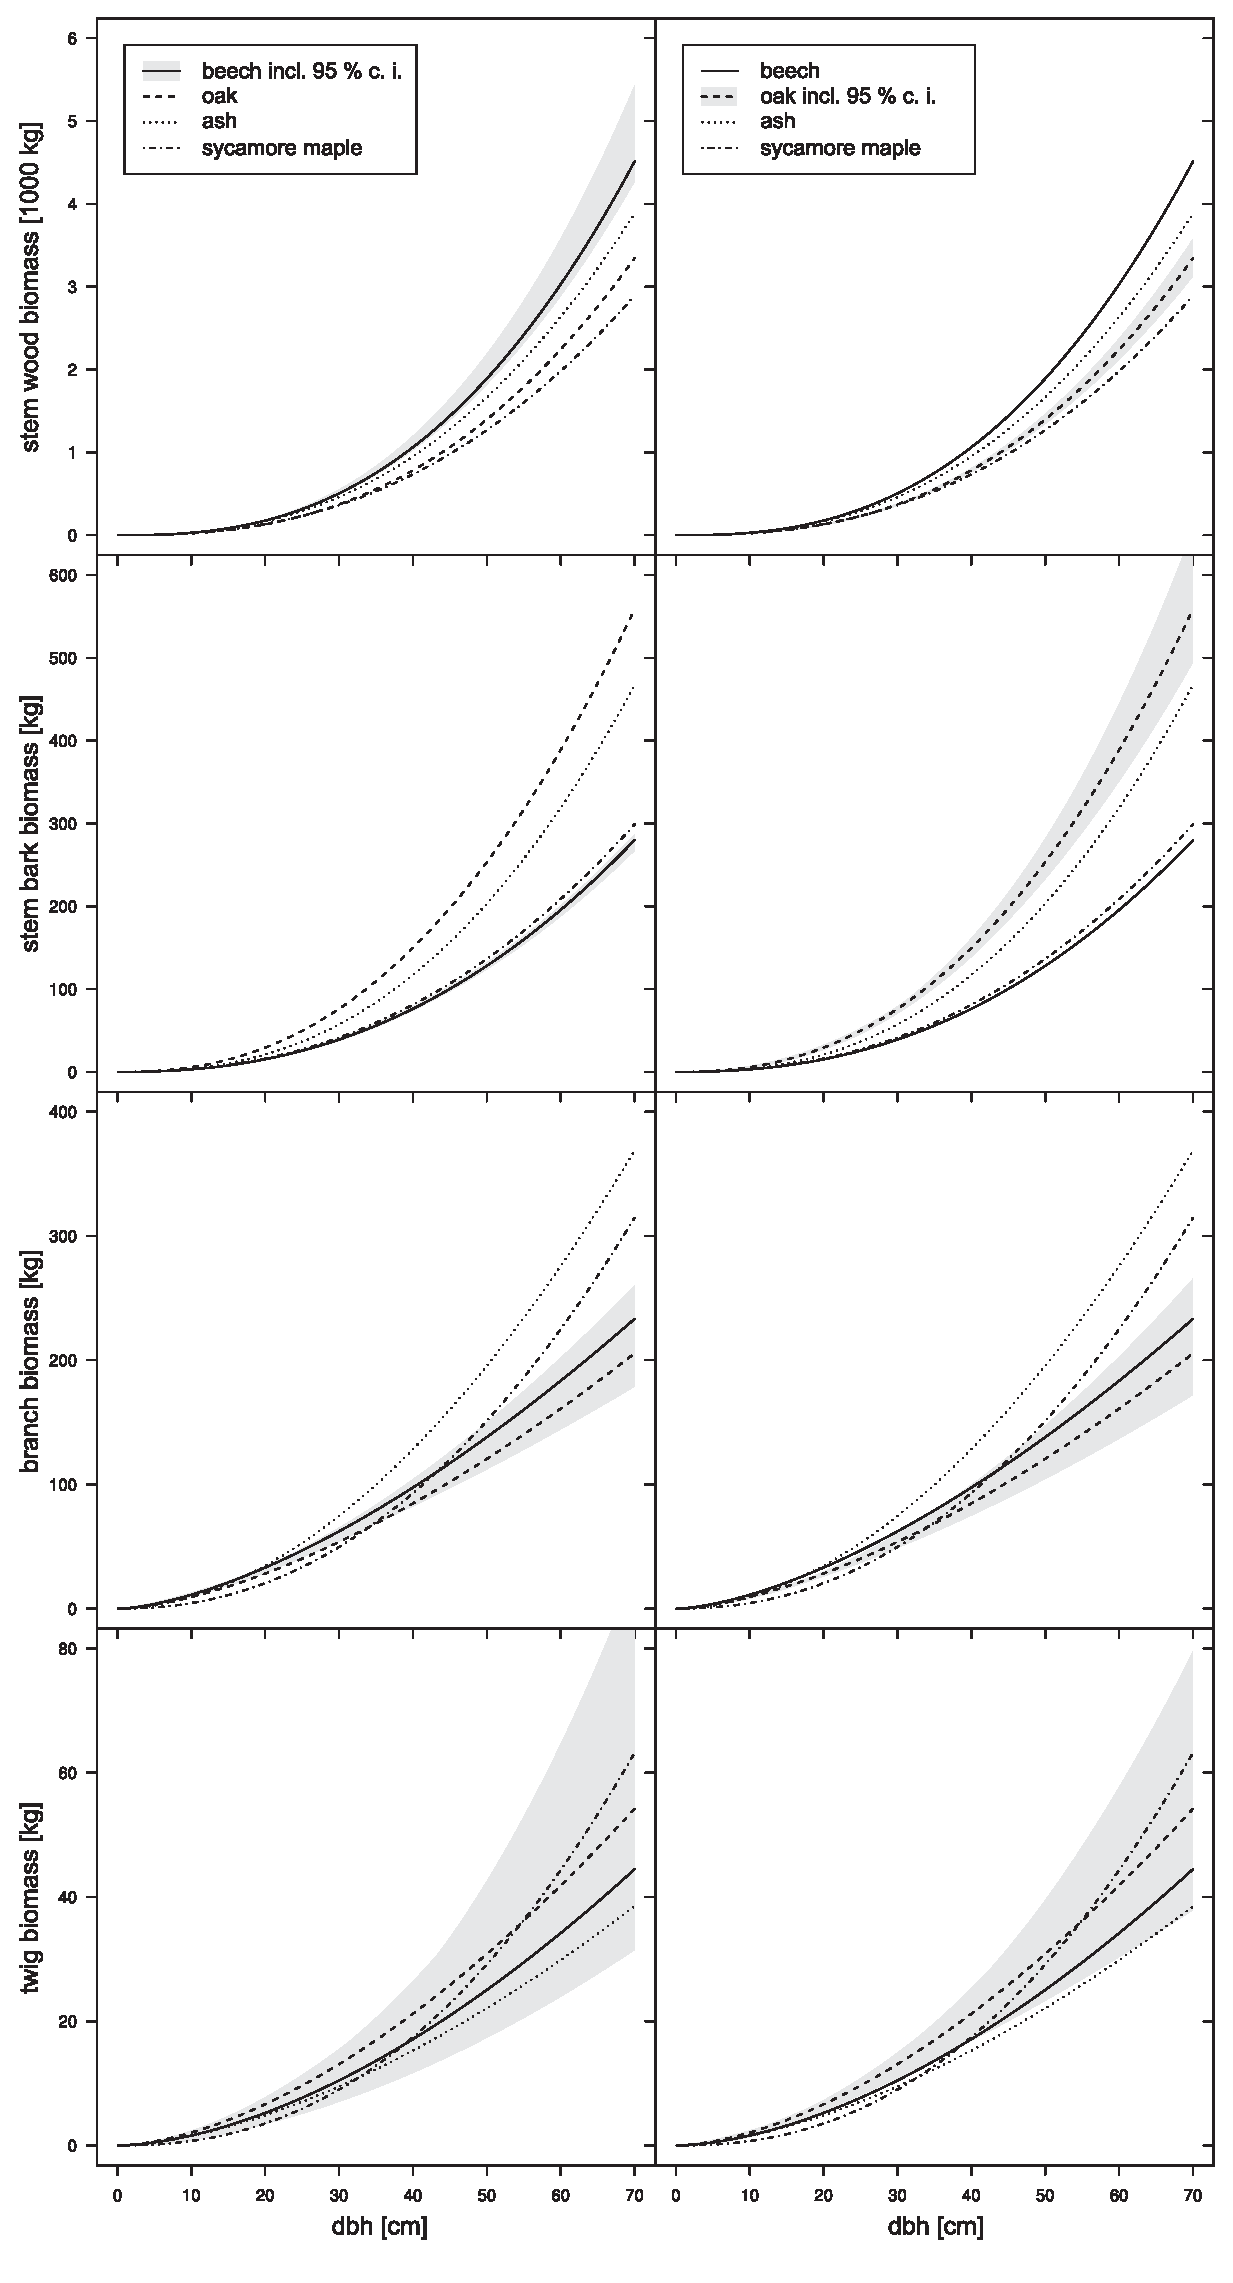
\includegraphics[width=0.75\textwidth]{Grafiken/bm/Fig_2_Regression_curves.eps}
	\caption{Regression of the biomass functions for European beech, oak, ash and sycamore over dbh. The left column includes a 95 \% confidence interval for the European beech regression function. The right column shows the same regression functions including a 95 \% confidence interval for the oak function.}
	\label{fig:bm:fig2}
\end{figure}

A comparison of the biomass models should show whether separate biomass functions for sycamore and ash are necessary. For this purpose confidence intervals were generated for the European beech and oak functions (Figure \ref{fig:bm:fig2}). We chose the 2-parametric functions with dbh as only descriptive variable for the model comparison. For stem wood there was no overlap across the whole spectrum of dbh. The curves of the stem wood functions of the 4 tree species ran more or less equidistant from one-another, with the European beech stem wood function lying above those of all other species. The lower confidence limit for the European beech stem wood function lay very near to the expected value. The European beech confidence interval had therefore no overlap with the other biomass functions. Although the oak stem wood function ran between the sycamore and ash functions, there was also no overlap with the other stem wood functions because the confidence intervals were comparatively narrow.

For the bark models there were also no areas of overlap between the graphs. The bark biomass functions could be separated into 2 groups. The graph of the sycamore bark biomass function ran very near to that of European beech. Due to the relatively large data pool and the small data variance, the confidence intervals for the European beech models were very narrow so, despite the proximity on the graph, there was no overlap with the sycamore function. The bark biomass functions for ash and oak lay almost twice as high on the graph as those of European beech and sycamore. The confidence interval of the oak function was much wider than the European beech confidence interval. The distance between the oak and ash functions is, however, so large that there was no overlap between the two.

The confidence intervals of the branch functions were altogether much wider than those of the stem wood and bark functions. The confidence interval of the European beech branch model enclosed the oak function and vice-versa. The sycamore function for branch biomass overlapped with the European beech confidence interval in the dbh range between 35 - 50 cm and with the oak function confidence interval in the range 30 - 45 cm. The graphs of the sycamore and ash branch biomass functions were, however, much steeper. Consequently there is a clear difference between the sycamore and ash branch models to the European beech and oak models.

The graphs of the 4 twig biomass models were indistinguishable over most of the value range. The confidence intervals of these functions were very asymmetric and even wider than the branch function confidence intervals. The confidence interval of the European beech function was the widest and enclosed all the other functions across the whole diameter range. The confidence interval of the oak function was slightly narrower and enclosed the European beech and sycamore functions from a dbh of ca. 40 cm and higher. The function graph of the sycamore function ran within the confidence intervals of both European beech and oak over much of the dbh value range. It was, however, much steeper than all other models. The graph of the ash function lies close under that of the European beech function. Consequently, the twig functions are mostly indistinguishable by means of the confidence interval analysis although their curvature is partially different.

The proportion of stem wood in the tree biomass increased disproportionately high with increasing dbh. For the oak functions the stem wood percentage increased sharply at first, from 56 \% by dbh 10 cm to 68 \% by dbh 20 cm. By dbh 60 cm the stem wood share of the biomass was 79 \% but did not increase much further after that. On average the stem wood share was 72 \%. The proportion of the bark biomass was more or less constant at ca. 14 \%. The share of branch as well as twig biomasses decreased with increasing dbh. The share reduced from 26 \% to 5 \% for branch and 4 \% to 1 \% for the twig biomass in the observed diameter range. The relationships between the tree fractions of the other tree species were comparable. The stem wood percentage for European beech increased from 78 \% to 89 \% in the diameter range 20 cm to 60 cm, that of sycamore from 77 \% to 81 \% and ash from 73 \% to 81 \%. For each tree species the stem wood share increases digressively and nears an asymptote. Above a dbh of ca. 60 cm the stem wood share in the tree species studied did not change much. The share of bark in the total biomass for European beech (6 \%) sycamore (9 \%), and ash (10 \%) remained relatively constant. The share of biomasses in branches and twigs thus also decreased with increasing dbh for those 3 tree species.

\begin{figure}
	\center
	\includegraphics[width=0.85\textwidth]{Grafiken/bm/Fig_3_Fraction_Biomass.eps}
	\caption{Biomass of the tree fractions in absolute scale (left) and relative to the total aboveground biomass (right) over dbh for oak.}
	\label{fig:bm:fig3}
\end{figure}

%%----------------------%%
%% Sensitivity analysis %%
%%----------------------%%
\subsection{Sensitivity analysis}
\label{subsec:bm:results:sensitivity}

In order to assess the magnitude of the effect that different biomass functions can have on results at the stand level, real and simulated test stands were used (Tables \ref{tab:bm:tab2} and \ref{tab:bm:tab4}). The sum of the total aboveground biomasses for all trees in these stands was firstly calculated with the tree species specific biomass functions. Then, secondly, the sum of the total aboveground biomasses was again calculated using only the oak biomass functions for estimating biomasses of sycamore and ash trees. The full tree biomass at the stand level for the first test stand (proportion European beech: 75 \%) was calculated to be ca. 200 t ha$^{-1}$ when using tree specific biomass functions. Using oak biomass functions for sycamore and ash led to a 4 \% overestimation of the stand biomass (ca. 7 t ha-1). The difference between the two calculation methods increased steadily with a decreasing proportion of European beech, reaching a maximum overestimation of 11 \% (21 t ha$^{-1}$) for a stand with an equal tree species mixture. If the proportion of European beech was held constant, then the difference of the total aboveground biomass on stand level increased with a decreasing ash percentage in the stand. In every case the estimated total biomass at the stand level was lower when separate, species specific, biomass functions were used.

\begin{table}[]
	\centering
	\caption{Sum of total aboveground biomass on stand level for stands with differing share of species. The biomass is calculated with distinct tree species specific biomass functions and also with oak biomass functions for ash and sycamore.}
	\label{tab:bm:tab4}
	\begin{tabular}{cccccc}
		\cline{1-3} \cline{5-6}
		\multicolumn{3}{c}{share {[}\%{]}}                                        &  & \multicolumn{2}{c}{total aboveground biomass {[}t ha$^{-1}${]}}                                                                                  \\ \cline{1-3} \cline{5-6} 
		\begin{tabular}[c]{@{}c@{}}European\\ beech\end{tabular} & ash & sycamore &  & \begin{tabular}[c]{@{}c@{}}tree specific\\ functions\end{tabular} & \begin{tabular}[c]{@{}c@{}}oak functions for\\ ash and sycamore\end{tabular} \\ \cline{1-3} \cline{5-6} 
		75                                                       & 12  & 12       &  & 199.4                                                             & 206.8                                                                        \\
		68                                                       & 25  & 7$^*$    &  & 201.6                                                             & 208.6                                                                        \\
		68                                                       & 16  & 16       &  & 199.0                                                             & 210.1                                                                        \\
		68                                                       & 7   & 25       &  & 194.5                                                             & 206.9                                                                        \\
		50                                                       & 25  & 25       &  & 197.3                                                             & 213.1                                                                        \\
		33                                                       & 33  & 33       &  & 188.1                                                             & 208.8                                                                        \\ \cline{1-3} \cline{5-6}
		\multicolumn{6}{l}{*Original test site (Table \ref{tab:bm:tab2})}
	\end{tabular}
\end{table}

%%-------------------%%
%% Nutrient contents %%
%%-------------------%%
\subsection{Nutrient contents}
\label{subsec:bm:results:nutrients}

In our analysis, the nutrient contents differed particularly between the tree species. In order to examine significant differences, we performed a parametric one-way analysis of variance for each nutrient and fraction combination with 5 \% significance level. The mean nutrients contents are listed in Table \ref{tab:bm:tab5}. All of the nutrient content data in the fraction and species groups were approximately normally distributed. For this, simple arithmetic group means are sufficient for data description and model building. This mean nutrients contents allows the tree and fraction specific calculation of the nutrients by multiplying its biomass with the respective element content from Table \ref{tab:bm:tab5}.

% Please add the following required packages to your document preamble:
% \usepackage{multirow}
\begin{table}[]
	\centering
	\caption{Group mean and standard deviation of nutrient content [g kg$^{-1}$] for the tree species European beech, oak, ash and sycamore. N: Observed number of trees.}
	\label{tab:bm:tab5}
	\begin{tabular}{ccccccccc}
		\hline
		spec.                                                                        & frac.                                                                & Ca           & Mg           & K            & C             & N            & P            & S            \\ \hline
		\multirow{8}{*}{\begin{tabular}[c]{@{}c@{}}oak\\ N=8\end{tabular}}           & \multirow{2}{*}{\begin{tabular}[c]{@{}c@{}}stem\\ wood\end{tabular}} & 0.729        & 0.100        & 1.131        & 495.898       & 1.895        & 0.087        & 0.126        \\
		&                                                                      & ($\pm$0.592) & ($\pm$0.090) & ($\pm$0.362) & ($\pm$6.515)  & ($\pm$0.736) & ($\pm$0.060) & ($\pm$0.038) \\
		& \multirow{2}{*}{bark}                                                & 26.350       & 0.768        & 2.363        & 484.346       & 6.518        & 0.276        & 0.622        \\
		&                                                                      & ($\pm$6.787) & ($\pm$0.401) & ($\pm$0.789) & ($\pm$45.123) & ($\pm$1.602) & ($\pm$0.090) & ($\pm$0.237) \\
		& \multirow{2}{*}{branch}                                              & 6.347        & 0.522        & 1.954        & 492.667       & 5.165        & 0.323        & 0.333        \\
		&                                                                      & ($\pm$2.882) & ($\pm$0.169) & ($\pm$0.223) & ($\pm$5.918)  & ($\pm$1.362) & ($\pm$0.091) & ($\pm$0.115) \\
		& \multirow{2}{*}{twig}                                                & 7.368        & 0.813        & 3.050        & 504.286       & 10.531       & 0.769        & 0.621        \\
		&                                                                      & ($\pm$2.727) & ($\pm$0.379) & ($\pm$0.395) & ($\pm$7.683)  & ($\pm$1.285) & ($\pm$0.089) & ($\pm$0.103) \\ \hline
		\multirow{8}{*}{\begin{tabular}[c]{@{}c@{}}beech\\ N=18\end{tabular}}        & \multirow{2}{*}{\begin{tabular}[c]{@{}c@{}}stem\\ wood\end{tabular}} & 0.968        & 0.302        & 1.135        & 493.686       & 1.492        & 0.100        & 0.091        \\
		&                                                                      & ($\pm$0.156) & ($\pm$0.132) & ($\pm$0.248) & ($\pm$6.100)  & ($\pm$0.520) & ($\pm$0.056) & ($\pm$0.016) \\
		& \multirow{2}{*}{bark}                                                & 22.738       & 0.517        & 2.351        & 487.684       & 6.855        & 0.351        & 0.331        \\
		&                                                                      & ($\pm$7.651) & ($\pm$0.191) & ($\pm$0.413) & ($\pm$22.248) & ($\pm$1.370) & ($\pm$0.093) & ($\pm$0.053) \\
		& \multirow{2}{*}{branch}                                              & 3.150        & 0.371        & 1.559        & 493.113       & 2.805        & 0.243        & 0.148        \\
		&                                                                      & ($\pm$1.536) & ($\pm$0.140) & ($\pm$0.309) & ($\pm$7.705)  & ($\pm$0.520) & ($\pm$0.124) & ($\pm$0.019) \\
		& \multirow{2}{*}{twig}                                                & 6.883        & 0.524        & 2.989        & 508.817       & 8.427        & 0.791        & 0.479        \\
		&                                                                      & ($\pm$2.839) & ($\pm$0.266) & ($\pm$0.569) & ($\pm$8.408)  & ($\pm$1.039) & ($\pm$0.297) & ($\pm$0.054) \\ \hline
		\multirow{8}{*}{\begin{tabular}[c]{@{}c@{}}ash\\ N=37\end{tabular}}          & \multirow{2}{*}{\begin{tabular}[c]{@{}c@{}}stem\\ wood\end{tabular}} & 0.823        & 0.193        & 1.654        & 493.495       & 1.448        & 0.092        & 0.113        \\
		&                                                                      & ($\pm$0.148) & ($\pm$0.08)  & ($\pm$0.313) & ($\pm$5.497)  & ($\pm$0.342) & ($\pm$0.036) & ($\pm$0.044) \\
		& \multirow{2}{*}{bark}                                                & 25.505       & 0.657        & 5.067        & 477.649       & 5.312        & 0.291        & 0.469        \\
		&                                                                      & ($\pm$7.428) & ($\pm$0.165) & ($\pm$1.397) & ($\pm$10.354) & ($\pm$0.644) & ($\pm$0.065) & ($\pm$0.071) \\
		& \multirow{2}{*}{branch}                                              & 4.815        & 0.319        & 2.524        & 492.675       & 2.988        & 0.228        & 0.245        \\
		&                                                                      & ($\pm$2.138) & ($\pm$0.079) & ($\pm$0.521) & ($\pm$5.58)   & ($\pm$0.647) & ($\pm$0.075) & ($\pm$0.061) \\
		& \multirow{2}{*}{twig}                                                & 8.691        & 0.83         & 6.344        & 491.191       & 8.359        & 0.769        & 0.73         \\
		&                                                                      & ($\pm$1.689) & ($\pm$0.202) & ($\pm$0.775) & ($\pm$5.982)  & ($\pm$1.175) & ($\pm$0.202) & ($\pm$0.091) \\ \hline
		\multirow{8}{*}{\begin{tabular}[c]{@{}c@{}}syca-\\ more\\ N=25\end{tabular}} & \multirow{2}{*}{\begin{tabular}[c]{@{}c@{}}stem\\ wood\end{tabular}} & 1.068        & 0.322        & 1.403        & 497.572       & 1.467        & 0.111        & 0.118        \\
		&                                                                      & ($\pm$0.26)  & ($\pm$0.129) & ($\pm$0.268) & ($\pm$3.725)  & ($\pm$0.186) & ($\pm$0.021) & ($\pm$0.021) \\
		& \multirow{2}{*}{bark}                                                & 25.184       & 0.861        & 3.784        & 474.982       & 7.737        & 0.57         & 0.772        \\
		&                                                                      & ($\pm$7.479) & ($\pm$0.21)  & ($\pm$1.027) & ($\pm$10.544) & ($\pm$1.502) & ($\pm$0.144) & ($\pm$0.134) \\
		& \multirow{2}{*}{branch}                                              & 4.089        & 0.491        & 2.394        & 493.285       & 3.403        & 0.318        & 0.283        \\
		&                                                                      & ($\pm$1.673) & ($\pm$0.122) & ($\pm$0.335) & ($\pm$4.084)  & ($\pm$0.654) & ($\pm$0.068) & ($\pm$0.059) \\
		& \multirow{2}{*}{twig}                                                & 9.668        & 0.815        & 3.889        & 495.799       & 9.948        & 0.898        & 0.709        \\
		&                                                                      & ($\pm$3.011) & ($\pm$0.227) & ($\pm$0.79)  & ($\pm$6.299)  & ($\pm$2.602) & ($\pm$0.268) & ($\pm$0.137) \\ \hline
	\end{tabular}
\end{table}

With ca. 500 g kg$^{-1}$ (dry biomass) in stem wood, as well as in bark, carbon has the greatest share of any element content in the entire dry weight. The average carbon content lies between 475 g kg$^{-1}$ and 509 g kg$^{-1}$, with slight differences between the tree species and fractions. In the stem wood sycamore differs significantly from beech while the carbon contents of other combinations do not differ significantly. In the bark fraction, ash and sycamore differ significantly from oak and beech. For sycamore and ash, the carbon content in the stem bark is a little lower than in the stem wood. The average nutrient contents, with the exception of a few calcium contents in the branches of sycamore and ash, were < 25 g kg-1. With few exceptions, the content of the various nutrients in wood can be ranked as follows: N > K > Ca > Mg > P = S. Ash has the largest potassium content (1.65 g kg$^{-1}$) of all 4 tree species. The potassium content in ash is throughout significantly higher than in all other examined species. In terms of the magnesium content, the trees can be separated into two groups. The mean content is significantly higher for sycamore and European beech than for oak and ash. Generally, the nutrient contents in bark are between 3 (N, P and K) and 25 (Ca) times higher than in wood. The concentrations of nitrogen, phosphor and sulfur in sycamore bark are always significantly higher than those of European beech and than those in the bark of oak and ash. The bark of ash has significantly lower nitrogen concentrations than the other species but higher potassium content.

\begin{figure}
	\center
	\includegraphics[width=1\textwidth]{Grafiken/bm/Fig_4_nutrient_eff_1.eps}
	\caption{Nitrogen (N), calcium (Ca) and potassium (K) nutrient response efficiency for European beech, ash and sycamore when harvesting stem wood (including bark) only in comparison to a full tree usage.}
	\label{fig:bm:fig4}
\end{figure}

The nutrient response efficiency per tree species was calculated for the European beech - broad leaf mixed test stand (Table \ref{tab:bm:tab2}). In Figures \ref{fig:bm:fig4} and \ref{fig:bm:fig5}, the results for the respective tree species and tree fractions are shown. The nutrient response efficiencies for stem wood usage were calculated by dividing the carbon concentrations in the fractions stem wood and bark by the respective nutrient concentrations. Analogously, the nutrient response efficiencies for full tree usage were achieved by dividing the carbon concentrations of all 4 fractions by the particular nutrient concentrations. With reference to potassium, calcium and sulfur, European beech had the most efficient biomass production and, therefore, the most efficient carbon sequestration rate. Ash had the lowest nutrient efficiency for calcium and potassium, while phosphorus was used just as efficiently by ash as by European beech. With reference to magnesium, ash was the most efficient species and sycamore the least, while there was no real difference in efficiency between the 4 tree species with regard to nitrogen.

\begin{figure}
	\center
	\includegraphics[width=1\textwidth]{Grafiken/bm/Fig_5_nutrient_eff_2.eps}
	\caption{Phosphor (P), sulphur (S) and magnesium (Mg) nutrient response efficiency for European beech, ash and sycamore when harvesting stem wood (including bark) only in comparison to a full tree usage.}
	\label{fig:bm:fig5}
\end{figure}

Because the branches and twigs are only used if the full tree is harvested, it seemed worth comparing the nutrient response efficiency of the stem wood biomass with that of the total aboveground biomass. The comparison revealed that the nutrient response efficiency of the total above ground biomass was always between 5 \% and 10 \% lower than that of the stem wood biomass. This trend can be observed for all examined tree species.



%%%%%%%%%%%%%%%%
%% Discussion %%
%%%%%%%%%%%%%%%%
\section{Discussion}
\label{sec:bm:discussion}

%%-------------------%%
%% Biomass functions %%
%%-------------------%%
\subsection{Biomass functions}
\label{subsec:bm:discussion:bm_functions}
In comparison to other existing function types, such as those of \citet{ledermann_2006}, \citet{eckmullner_2006} and \citet{marklund_1988}, the biomass model from \citet{hochbichler_2006} (Equation \ref{eq:bm:eq1}) proved, after extensive AIC and residual analyses, to be the most suitable. The model was fitted directly nonlinear without data transformation. There was thus no need for a subsequent bias correction \citep{baskerville_1972, smith_1993}. Due to the sufficiently large data pool the entire bandwidth of forestry relevant tree dimensions is covered by our biomass functions. A mixed effect regression model with distinct error structure for regional clusters did not improve our models. We therefore did not consider any mixed effect.

In large parts, the quality of the models depended on the tree fraction being examined (Table \ref{tab:bm:tab3}). The branch and twig models showed a higher variation in comparison with the stem wood and bark models. The accuracy of estimation of all stem wood and bark models could, though, be improved by including tree height in the models. If the appropriate data is available, then these more complex models are preferable. This was confirmed performing analysis of AIC, $v(\hat{y})$ and $r_{LR}^{2}$ (Table \ref{tab:bm:tab3}).

The nonlinear pseudo-r-squared can be interpreted as the proportion of explained variation. There are, nevertheless, unlike the linear r-squared, several possibilities of calculating it \citep{magee_1990}. The likelihood-ratio pseudo-r-squared $r_{LR}^2$ are thus often not directly comparable to the r-squared of other studies. It, however, becomes apparent that our r-squared are roughly in line with all r-squared found in literature (see e. g. \citet{zianis_2005} for a broad overview). In most other studies the r-squared of the stem and bark models amount at least to 0.9. The same appears for the branch and twig models. With values ranging from 0.6 to 0.8, the r-squared are much smaller.

Other studies \citep[e. g.][]{ledermann_2006, pretzsch_2014} have shown that other variables could also improve model accuracy. Including tree height, tree height at crown base, crown width, tree age and a dummy code for forked tree lowered model standard error for the European beech biomass model by ca. 6 \% and the oak model by ca. 13 \%, when compared to the dbh-only model in a study of \citet{ledermann_2006}. These results couldn�t be replicated in this study. Only tree age led, in a few cases, to a significant, though very small, model improvement. The age of individual trees is, however, seldom surveyed in the practice, so age was not further considered in creating the models. \citet{hochbichler_2006}, who developed branch biomass functions for oak and European beech, observed a slight model improvement of the beech model when using the crown ratio as additional independent variable. We were not able to reproduce this result with our data. The crown ratio was not significant in any model. The same was found for the tree height to tree diameter ratio. As we collected our data in pure stands under standard regimes, the influence of the mixture and concurrence on the allometry, as it was e. g. observed by \citet{pretzsch_2012}, could not be analysed.

Using a simple nonlinear regression for the tree fractions meant that any within-species correlation (collinearity) between fractions was not taken into account. This is of course a simplification. Since collinearity would have led to a huge difference between the distinct coefficients of variation and the combined coefficients of variation and we observed only minor differences (Table \ref{tab:bm:tab3}), it becomes clear that collinearity in the model had no considerably negative effect on any model. The combined model coefficients of variation were primarily influenced by the stem wood and bark models, variation in the branch and twig models had very little influence. There was thus only high correlation between fractions with comparatively low variation. The highest impact of collinearity was found for the sycamore biomass functions. The dimension of the combined coefficient of variation, however, was still very small. It can therefore be assumed that collinearity did not limit the validity of any model. Further analyses with simultaneous regression methods, such as a Seemingly Unrelated Regression \citep{henningsen_2007} or Restricted Regression, could establish whether the model error could be further reduced by considering collinearity during the regression. At any rate, the results of the analyses undertaken here indicate a valid estimation of the model parameters. Simultaneous methods could probably reduce the model variance significantly. Other studies, for instance \citet{sanquetta_2015}, came to the same conclusion. Using tree growth data they were able to show that the parameter estimations were close to the results when using both separate and simultaneous estimations, whereas the variance, and with it the model efficiency, could be improved by using simultaneous methods.

Due to the relatively small variance in the raw data, the confidence intervals for the stem wood and stem wood bark functions were, as expected, narrower than the confidence intervals for the branch and twig models in the model comparison (Figure \ref{fig:bm:fig2}). Owing to the very wide confidence interval calculated for the European beech twig function, it is only for the twig models that the biomass functions of other species overlapped with the European beech confidence interval. Because of the relatively large scattering of the twig (see also Table \ref{tab:bm:tab3}), the sycamore and ash twig functions could be substituted by the European beech function. The curve of the sycamore function, however, differed markedly from the other function curves. It should also be noted, that the twig biomass makes up only a small proportion of the total biomass.

The functions were compared using the 2-parameter models, with dbh as the single covariate, revealing clear differences in the biomass models. Using 3-parameter models, with tree height included as an additional variable, would reveal at least the same model differences. The addition of other significant variables would narrow the confidence bands even further, due to the reduced variance (Table \ref{tab:bm:tab3}). In conclusion, the comparison of the biomass functions obviously underlines the need for separate sycamore and ash functions. The biomass functions of these species differ clearly from the beech and oak functions. The estimation of single tree biomass for sycamore and ash using biomass functions for other tree species, which up to now has been the norm, certainly leads to biomass estimation errors.

The proportion of stem wood increases with increasing dbh (Figure \ref{fig:bm:fig3}). This increase in the stem wood proportion with increasing dbh could also be documented for European beech in the diameter range 6 - 16 cm by \citet{grote_2003}. They observed an increase of the average stem wood proportion from 30 \% to 80 \%, which is very close to the results from this study (Figure \ref{fig:bm:fig3}) for that diameter range. The data used by \citet{grote_2003} were sampled in a mixed oak - pine stand, which indicates that the relationship of stem wood biomass is similar in these stands, at least in the diameter range 6 - 16 cm. \citet{konopka_2015} also recorded an increase in the stem volume of young European beech up to 4 cm dbh, while \citet{cienciala_2005} and \citet{pretzsch_2014} observed a stem wood share between 70 \% and 90 \%, with a mean of 82 \%. This mean share is also similar to the data from this study (Figure \ref{fig:bm:fig3}), though neither of these 2 studies found a significant diameter trend. \citet{genet_2011} observed a shifting of the stem wood share from 60 \% to 75 \% in trees between 13 and 81 years old, which is also consistent with the results of this study. The stem wood bark percentage from our study of 6 \% is consistent with all values found in the literature \citep[e. g.][]{altherr_1978, grote_2003, pretzsch_2014}. The fraction proportions of oak also showed a diameter trend. The stem wood proportion has a rising tendency, but lies clearly under the stem wood proportion of European beech. The stem wood percentage of 68 \% to 80 \% in the 20 cm to 60 cm diameter range corresponds well with the data from \citet{pretzsch_2014}, who observed a mean percentage of 75 \%. \citet{grote_2003} observed an increase of the stem wood percentage from 61 \% to 71 \% in the dbh range 10 cm to 30 cm, which is again very close to the results presented here. The bark proportion is also consistent with the literature values \citep{altherr_1978, pretzsch_2014}, whereby \citet{altherr_1978} found a site dependency. Comparison of the fractions relations of ash and sycamore with literature functions were, due to differing fractionations, not possible. Comparison of the total aboveground biomass reinforces the validity as well as the importance of our models. It could be seen that our functions were slightly different to all other models found in the literature \citep{albert_2014, alberti_2005, bunce_1968}. As an example, our ash as well as our sycamore functions lay in between the functions of \citet{albert_2014}, who parameterized distinct functions with trees from a rich and a poor coppice stand. Although there are differences in the parameter estimations between the new parameterized functions in our study to former studies, the general proportions seem to be consistent with other biomass functions for all 4 tree species. This was expected as biomass functions are known to have regional differences \citep{cerny_1990, thurnher_2013}. Publishing specific biomass function for the northern and central part of Germany seems thus to be worthwhile for all 4 species.

%%----------------------%%
%% Sensitivity analysis %%
%%----------------------%%
\subsection{Sensitivity analysis}
\label{subsec:bm:discussion:sensitivity}
Biomass of ash and sycamore must recently be estimated by biomass function of other species. To assess the magnitude of the effect these false estimations can have on biomass estimations in the praxis, test stands were generated (Tables \ref{tab:bm:tab2} and \ref{tab:bm:tab4}). The oak biomass function was preferred to the European beech function for these analyses, because the curve of the oak function was a better fit with the sycamore and ash function curves (Figure \ref{fig:bm:fig2}). The results reinforce the need for separate biomass functions. As observed before, especially the sycamore functions were different to the oak biomass functions. In particular for sycamore the estimate was substantially improved with a separate species specific biomass function. In stands with a high proportion of sycamore, estimating biomass using oak functions led to massive overestimation of the biomass and the sequestered carbon (Table \ref{tab:bm:tab4}). The same effect would also be evident in the products of forestry use and the downstream transport chain. The actual biomass potential would be considerably lower than the predicted potential. With respect to the fact that accurate biomass predictions are mandatory for a reliable biomass potential estimation, this underestimation, as it was obligatory until now, seems not to be acceptable.

%%-------------------%%
%% Nutrient contents %%
%%-------------------%%
\subsection{Nutrient contents}
\label{subsec:bm:discussion:nutrients}
Varying nutrient contents, not only between tree species but also between tree fractions, has been demonstrated in many studies for European beech and oak before \citep[e. g.][]{augusto_2000, muller-using_2004, pretzsch_2014}. In this study these differences in nutrient content were also shown for sycamore and ash (Table \ref{tab:bm:tab5}). In comparison to European beech and oak, ash and sycamore species have significantly higher calcium and potassium contents and significantly less carbon contents. Export of sycamore and ash biomass will thus be underestimated, if European beech or oak contents are used for their estimation. In other studies \citet[e. g.][]{joosten_2003}, it was shown that nutrient contents also significantly depended on the site quality. As sycamore and ash only grow on sites of relatively high quality, our sample for the chemical analysis comprised rich stands only. The stand quality thus had of course no significant explanatory content in our study. The nutrient contents are generally higher in the bark than in the wood and this applies to all 4 studied tree species. Because the proportion of bark within a tree decreases with increasing branch diameter, small diameter wood fractions (branches and twigs) have higher nutrient concentrations.

This is reflected in lower nutrient response efficiencies for these fractions \citet{vitousek_1982, rumpf_2011, meiwes_2012}. A greater amount of nutrients has been used in building biomass in these smaller fractions than are needed to build the same biomass in stem wood. Except for nitrogen, the calculated nutrient response efficiencies were substantially different for the observed tree species. This again reinforces the need for distinct biomass and nutrient content models. It must, however, be considered that our definition of the nutrient efficiency is slightly different to the original definition by \citet{vitousek_1982}. He stated that in long-living perennial plants the nutrient efficiency calculates as the inverse of the nutrient concentration in the wood increment, the litterfall and the root turnover. As none of those variables was measured in our study and because the litterfall as well as the root turnover remain in the stand, their efficiency is not relevant for the calculation of the biomass potential. We thus only focused on the nutrient content of the aboveground biomass. The use of small dimensioned wood leads to a disproportionately high nutrient loss and has a greater negative effect on the nutrient supply of the site than stem wood harvest alone \citep{block_2012, meiwes_2012, pretzsch_2014}. On the other hand, in times of modern processing methods, in precisely those recently often unused wood fractions there is a huge potential for the bio-based industry.

%%%%%%%%%%%%%%%%%
%% Conclusions %%
%%%%%%%%%%%%%%%%%
\section{Conclusions}
\label{sec:bm:conclusions}
When coupled with individual site information, the results of this study help determining the optimal biomass potential of mixed stands with European beech, oak, sycamore and ash. In forest stands with homogeneous tree species and age distributions the biomass and nutrient quantities could certainly be estimated with sufficient accuracy using stand parameters such as mean basal tree area \citep{pretzsch_2014}. As is made clear by the example in Table \ref{tab:bm:tab4}, this is not possible in mixed broad-leaf stands. The use of the oak biomass function for all tree species would lead to overestimating both biomass and nutrient quantities. Because the share of multiple layer, species-rich stands in forests is increasing \citep{ti_2014}, and will probably continue to increase \citep{bmel_2014}, the need for species specific biomass functions becomes ever more urgent. For estimating the optimal site specific harvest quantities, biomass functions, and knowledge of tree fraction nutrient content, for the tree species sycamore and ash are a useful addition to already existing functions, and could help to enable the full biomass potential of the forest to be exploited in the future. They improve the planning security of forestry activities and of all further processes in the biomass supply chain and help to analyse the trade-off between usage intensity and site sustainability. All further analyses that require reliable biomass estimations, for example supply analysis for operative and strategic planning or carbon inventories, will also profit from the biomass functions introduced here. The introduced models can help gathering the huge biomass potential from long-term broad-leaf stands that was unused till now \citep{ti_2014}.

%%%%%%%%%%%%%%%%%%%%%%
%% Acknowledgements %%
%%%%%%%%%%%%%%%%%%%%%%
\section*{Acknowledgements}
\label{sec:bm:acknowledgements}
The authors are grateful to the Project Management J�lich of the Federal Ministry of Education and Research for funding this research through the projects \textit{BEST} (003L033F) and Cluster \textit{Bio-Economy} (031A294) as well as to the Agency for Renewable Resources of the Federal Ministry for Consumer Protection, Food and Agriculture for funding the project \textit{M�glichkeiten und Grenzen der Vollbaumnutzung} (22015407). We would like to thank the anonymous reviewers for their helpful and constructive revision of the manuscript.
